\documentclass[11pt,titlepage]{book}
\usepackage{times}
\usepackage[pdftex]{graphicx}
\DeclareGraphicsExtensions{.jpg,.pdf,.mps,.png}
\usepackage{color}
\usepackage{listings}
\usepackage{ifthen}
\usepackage{alltt}
\usepackage[raiselinks=true,pdfpagemode=None,pdfview=FitB]{hyperref}

\lstloadlanguages{C++,Java}
\definecolor{codecolor}{rgb}{0,0,.3}
\lstset{basicstyle=\small,
        frame=tb,
        escapechar=\`}
\def\thelstlisting{\thesection.\arabic{lstlisting}}

% \fxl{k} place a pale yellow box behind the next k lines
\def\fxl#1{%
\newdimen\fxlheight\setlength{\fxlheight}{#1\baselineskip}%
\advance\fxlheight by -0.5\baselineskip%
\begin{picture}(0,0)%
\setlength{\unitlength}{\baselineskip}%
\put(0,0){\makebox(0,0.75)[tl]{%
\colorbox{paleyellow}{%
\rule{0pt}{\fxlheight}%
\rule{\linewidth}{0pt}}%
}}\end{picture}%
}
\definecolor{paleyellow}{rgb}{1,1,.75}




\addtolength{\oddsidemargin}{-0.5in}
\addtolength{\evensidemargin}{-0.5in}
\addtolength{\textwidth}{1.0in}
%\addtolength{\topmargin}{-0.5in}
%\addtolength{\textheight}{1.0in}

\newcommand{\algae}{{\sc AlgAE}}
\newcommand{\cpp}{{\tt C++}}
\newcommand{\cd}[1]{{\tt #1}}


\newcommand{\Label}[1]{\label{#1}}
%\newenvironment{code}{\begin{alltt}}{\end{alltt}}


\begin{document}

\title{AlgAE \\ (Algorithm Animation Engine) \\ Reference
Manual\\Version 3.0}
%\thanks{This document is also available online at
%{\tt http://www.cs.odu.edu/\string~zeil/algae/refmanht/refmanht.html}.}}
\author{Steven J. Zeil \\
Old Dominion University \\ Dept. of Computer
Science}
\date{August 20, 2011}

\maketitle


{\bf Copyright:}
This document, and the \algae\ source code, is\\
\begin{center}
\copyright{} 2011, Steven~J.~Zeil.
\end{center}
\pagenumbering{roman}

Permission is granted to freely distribute this document and the
associated source code and to prepare derivative works, providing that
the original copyright notice is retained.

The \algae\ system is distributed free of charge as a service to other
instructors. I make no warranty about its correctness (except to
assert my professional opinion that, like most software, it probably
does contain bugs) or its suitability to any specific application
(except to state that I myself have found it very useful indeed).

I welcome bug reports and suggestions for improvements, but ask you to
understand that this is not my research or instructional focus, and I
cannot promise a timely response.

If these terms are unacceptable to you, or if you live in a legal
jurisdiction that prohibits such waivers of warranty, then please do
not use this software.  On the other hand, if you can live with these
terms, then I hope that you find \algae\ useful.

\noindent
SJZ
\vfill
\newpage

\tableofcontents

\newpage
\chapter{Introduction}
\section{What is AlgAE?}
\pagenumbering{arabic}

\algae\ is a framework for quick construction of algorithm
animations. \algae\ is aimed at CS instructors who
employ projection screen monitors, LCD overhead pads,
or other devices to display computer video
output in the classroom or who publish web content in support of their courses.
\algae\ allows the instructor to take
typical \cpp\ or Java code from a course's textbook or lecture notes and, with
relatively little effort, produce an ``animated'' version of that
code. These animations will show the data as it is being manipulated by
the code. Data is portrayed as a collection of labeled boxes
connected by arrows (denoting pointers). \autoref{session} shows a
typical \algae\ animation in progress.
\begin{figure}
\centering
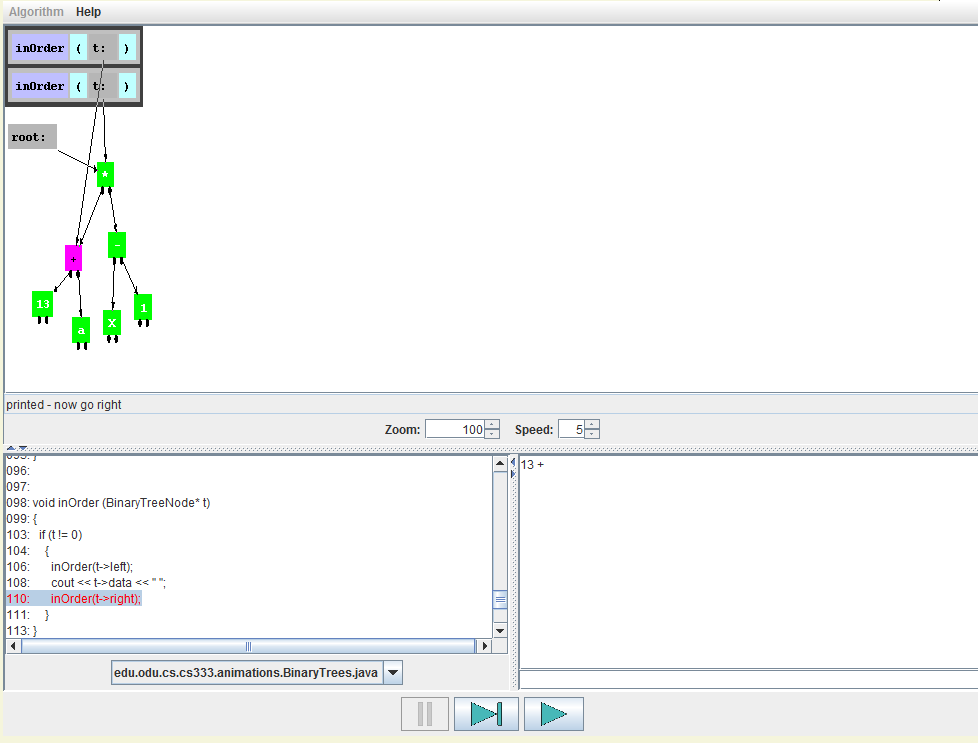
\includegraphics[width=\textwidth]{images/screenshot}
\caption{A Typical AlgAE Animation in Progress}
\label{session}
\end{figure}

I have used \algae\ (and an earlier version, written in
Pascal)  for our CS2 course (which emphasizes program design, the use
of ADT's, and some fundamental data structures) and  for a course in
Advanced Data Structures and 
Algorithms.  I have used it with LCD overhead pads, external video
projectors, and scan converters feeding into a broadcast TV signal.
%\footnote{Old Dominion University has a very active {\em Teletechnet}
%program providing interactive televised course offerings at community
%colleges, libraries, military bases (and an occasional Navy ship out
%at sea!), and other sites.}
 \algae\ animations have been an integral part of a
\href{http://www.cs.odu.edu/~fac/teched.html}{data structures}
course that I offer to distance students via the internet for more 
than 10 years.

Version 3.0 of \algae\ is a major rewrite of the original system. It
is easier to install and to use than the earlier versions.\footnote{On the
other hand, direct animation of C++ code is no longer supported
(though it is relatively easy to use Java to simulate animation of
C++). The network socket-based architecture used to support C++
animation by Versions 1 and 2 was unwieldy --- many people found it
hard to install, and University network administrators are
increasingly reluctant to open up ports for software that they
themselves do not maintain.

I hope to restore C++ support in the near future.}



\section{Design Principles}

\algae\'s design is based on the following principles:
\begin{itemize} 
\item[] {\em Animations should be tied to real, running code.} Yes,
there are lots of general-purpose animation packages out there that
can produce much prettier pictures. Or you can simply use a
conventional drawing tool to present a series of ``snapshots'', slide
by slide.  Both of these approaches require you to script out, before
the lecture, the exact sequence of operations you want to show. I find
this takes more time, in the long run, than building an \algae\
animation. In particular, I found that small mistakes in a ``script''
often meant having to go back and redraw large numbers of frames.

Perhaps the biggest drawback to these scripted approaches is the lack
of flexibility.  You can walk nicely through a scripted presentation
of the algorithm's execution, then a student raises a hand, and asks
``but what if\ldots'' and takes you right out of your script. With
\algae\, you simply re-run the algorithm with different inputs.


\item[] {\em Animations should be tied to code from the course text
and lecture notes.}  Instructors who are facile with graphics-rich
languages and packages might consider simply writing a program to draw
pictures that simulate the algorithm being discussed. But I suspect
that this, also, will prove more time-consuming than using
\algae. Furthermore, this alternative introduces the problem of
keeping the the animated algorithm consistent with the code under
discussion.  It's counter-productive to have the animation do things
in a different order than can be explained by students reading along
in their notes on the algorithm.

\item[] {\em It must be easy to create an animation from existing
code.} This is essential, because otherwise it would be more effective
for an instructor to fall back on hand-drawn illustrations. 
Also, texts change frequently, and so, therefore, does the code to be
presented to the students. (A year
after I finished my Pascal animations, our Department changed our
instructional programming language to \cpp. Since that change, I've
used 3 different data structures texts, and many of my other texts
have come out with new editions.) 

\item[] {\em The animations must be easy to run and control.} When I'm
lecturing, I don't need the distraction of trying to manage a
complicated interface while still trying to keep my speech coherent. 
Also, students frequently ask if they can run the animation programs
themselves while studying outside of class.

\item[] {\em Some sort of automated layout is essential.}  In my
earlier Pascal algorithm animator, each object had to be manually
positioned using the mouse. This turned out to be terribly
distracting, especially for data structures like AVL trees where the
``natural'' positions of objects changes regularly.

\item[] {\em The instructor/student needs constant feedback about where the
current execution point is in the algorithm.} Without this, it's too
easy to get confused and totally demolish the instructor's reputation
for infallibility!  \algae\ provides both a status area for
instructor-designed messages, and an ability to synchronize a view of
the source code with the current execution location.  The ability to
trace through the source code is shown in \autoref{session}. If a
sufficiently large font size is selected for this trace, students can
read the algorithm code off the 
screen, though I usually prefer to have them follow along on hard copy,
using the trace window to keep myself on track.

\item[] {\em You don't need to show lots of objects on the screen at
  once, but you do sometimes need to make them large.} For
  instructional purposes, a couple dozen objects on the screen at once
  seems to be more than enough. Consequently, \algae\ does not place
  much emphasis on speedy rendering of large numbers of objects. On
  the other hand, for the text in these objects and their connecting
  pointers to be visible in a large lecture room or on a conventional
  TV monitor (conventional TV bandwidth imposes some pretty severe
  constraints on text presentation and line drawing), you often need to
  make everything quite large.

%\item[] {\em Make the most of the screen real estate.} If objects have
%to be drawn large, you can't fit very many on the screen, so screen
%area becomes a precious commodity.  I've adopted a rather spartan look
%for these programs (no toolbars, keep the status line simple and
%small, etc.) to keep as much room available for the main picture as
%possible.
\end{itemize}

\section{Platforms Supported}

Version 3.0 of \algae\ software is written entirely in Java and should
be executable on almost any system. Animations created using
\algae\ can be distributed and run as standalone applications or
posted as Java web applets.

The current version is compiled using Java 6. The project build is
supported using Apache's \texttt{ant}\cite{Apache/ant}.


\chapter{Installation}

\section{Obtaining \algae}

\algae\ is available \href{ftp://ftp.cs.odu.edu/pub/zeil/algae/algae-3.0.zip}{via anonymous ftp} at {\tt ftp.cs.odu.edu} in the
directory {\tt /pub/zeil/algae}.



\section{Configuration and Installation}

\newcommand{\Root}{{\em algae-root}}
\newcommand{\Platform}{{\em platform}}

\begin{enumerate}
\item Unpack the \algae\ {\tt .zip} file into a directory of your
choice.  For the sake of exposition, I will assume throughout this
section that you have chosen to place this in a directory named
\Root. 

\item You will need a copy of the Sun Java Help library, \texttt{jhbasic.jar} \cite{Sun/help}. If one is not included in the \Root\texttt{/AlgAE} directory, find a copy on the net and place it there.

\item In the \Root\texttt{/AlgAE} directory, run
\begin{alltt}
ant
\end{alltt}
This should build the \texttt{AlgAE.}\textit{versionnumber}\texttt{.jar} file containing the Java engine.


\end{enumerate}



\section{Testing your installation}

The installation includes various sample animations of both Java and
\cpp\ code.  The Java animations will be found in the \Root\ directories other than the main \Root\texttt{/AlgAE} directory.

You should be able to compile any of these by giving the command
\begin{alltt}
ant
\end{alltt}
and to execute them by giving the command
\begin{alltt}
ant run
\end{alltt}


\chapter{Running an Animation}

When an \algae{} animation is launched, you will be presented with a
blank animation window. From the {\tt Algorithms} menu, you can select
any of several operations you would like to perform, e.g., inserting
an item into a binary search tree, removing an item, do a post-order
traversal, etc.

At selected points in the algorithm, the program will pause and draw a
picture of the current data state. The picture in
\autoref{session} is an example of this.

Boxes in the picture that represent data allocated on the heap can be
repositioned by dragging them with the mouse, if you are unhappy with
the automatic layout.

The controls below the main drawing area should be reminiscent of a
CD/DVD player. You can move forward one step at a time, or move
continuously without pausing. You can also ``rewind'' an animation to
re-examine details that you might have missed.


That's basically all there is to it.   More details on the available
commands and options may be obtained via the ``Help'' menu.




\section{Deploying an Animation}\label{deploying}

The most common way to deploy an animation is as an applet.

For this purpose, you will need 4 things:
\begin{enumerate}
\item The compiler \algae\ engine, \texttt{AlgAE.}\textit{version}\texttt{.jar}
\item The Sun Java Help library, \texttt{jhbasic.jar}
\item A jar file (or collection of class files) representing your specific animation, and
\item An HTML file that invokes the animation as an applet.

Typically, this will contain an applet element similar to the following
\begin{lstlisting}[language=HTML,frame=tb]{}
  <applet
     code="`\textit{yourAnimationMainClassName}`"
     archive="`\textit{yourAnimationName}`.jar,
               ../AlgAE/AlgAE.3.0.jar,../AlgAE/jhbasic.jar"
     width=10 height=10 
     alt="Is Java disabled on this browser?">
Oops.
This browser does not display Java applets.
   </applet>
\end{lstlisting}
Of course, you will need to adjust the paths to the \algae\ and \texttt{jhbasic} jars according to your own preference.

By default, \algae\ applets will pop up as a separate window when the page 
is visited. If you prefer to have the animation display within the page, add the \texttt{inline} parameter and give a sufficiently large height and width:
\begin{lstlisting}[language=HTML,frame=tb]{}
  <applet
     code="`\textit{yourAnimationMainClassName}`"
     archive="`\textit{yourAnimationName}`.jar,
              ../AlgAE/AlgAE.3.0.jar,../AlgAE/jhbasic.jar"
     width=800 height=700 
     alt="Is Java disabled on this browser?">
     <param name="inline" value="1"/>
Oops.
This browser does not display Java applets.
   </applet>
\end{lstlisting}
\end{enumerate}

Place these in a webserver-accessible directory and publish the URL of the HTML page.







\lstset{basicstyle=\small,
        frame=tb,
        escapechar=\`}


\chapter{Animating a Java Algorithm}

This section presents the major capabilities of \algae\ via a series
of examples. 


\section{Animation with Arrays}\label{sortingExample}

The first example will be relatively simple, because most of 
the rendering decisions will correspond to \algae's built-in defaults.

Our starting point will be the Java class in \autoref{list:sortingStart}, which 
contains three well-known sorting algorithms.
\lstinputlisting[language=Java,frame=TB,caption={An ADT for Disjoint Sets\label{list:sortingStart}}]{src/edu/odu/cs/AlgAE/Demos/Sorting0.java}

\begin{itemize}
\item You can place your code in any package you wish, or forgo a
  package entirely.  I place my copy in {\tt edu.odu.cs.AlgAE.Demos}
  because I wish to make it part of the \algae\ distribution.  You
  should probably not use a more appropriate designation for your own
  work.

\end{itemize}


\subsection{Setting Up An \algae\ Project}

The first step is to set up a project structure. I recommend using
\texttt{ant}\cite{Apache/ant} as the main project manager, though it's
often convenient to do the bulk of the work in an
\texttt{ant}-friendly IDE such as Eclipse \cite{Eclipse}.

\begin{enumerate}
\item Create a directory for the project. Within that project directory 
create a \texttt{src} directory to hold your Java code.

\item Then, within the project directory, create a \texttt{build.xml} file for \texttt{ant}. \autoref{list:buildxml} shows a possible structure.
\lstinputlisting[language=HTML,frame=TB,caption={Ant Build File, build.xml\label{list:buildxml}}]{build.xml}
\begin{itemize}
  \item Change the project name and description as desired.
  \item The \texttt{project} property is used to name the final Jar file
    produced as the output.
  \item The \texttt{mainClass} property names a Java class that will be
    the default animation driver to be executed in the produced Jar file.
    It will also be run by the
\begin{alltt}
ant run
\end{alltt}
    command.
    
    Note that a project (and hence the project's Jar file) can actually have
    several animations. This property establishes only a default selection.

  \item The \texttt{version} and \texttt{AlgAE.dir} properties are sued 
    to locate the already compiled \algae\ library and the accompanying
    \texttt{jhbasic.jar} file.

  \item The remainder of the file can, for most simple animations, be left
    unchanged.
\end{itemize}

If setting up a project directory with Eclipse \cite{Eclipse} or other
project managers, be aware that a deliberate design decision is to
place the compiled class files into the same directories as the source
code. Although this practice is often discouraged in large projects,
individual \algae\ animations are seldom large. More importantly, the
feature of displaying the code being animated exploits this decision
to locate the relevant source code file.

\item Next, create an HTML file (or several files) to invoke the
  animation(s) in the project, as per the guidelines in
  \autoref{deploying}. \autoref{list:html} shows an example of such a
  file. I typically include basic instructions to the students telling
  them what kinds of activities they might employ to explore the
  animation.
  \lstinputlisting[language=HTML,frame=TB,caption={HTML Applet Support\label{list:html}}]{index.html}

\item Finally, add (or build) your animation source code within the
  \texttt{src} directory. As with all Java code, if your classes are
  declared inside packages, you will need to construct the directory
  structure corresponding to the package structure.
\end{enumerate}

\subsection{Creating the Driver}

Each \algae\ animation starts its execution from a {\em driver}. The
driver must be a subclass of
\texttt{edu.odu.cs.zeil.AlgAE.Animation}. {\tt Animation} itself is a
subclass of {\tt JApplet} and therefore can be run as a web applet. It
also, however, provides support for being run as a standalone
application. This is often more convenient during development and debugging.

The basic structure of a driver is shown below:
\begin{lstlisting}[frame=tb,language=Java]{Driver Structure}
package edu.odu.cs.AlgAE.Demos;


import edu.odu.cs.zeil.AlgAE.Animation;
import edu.odu.cs.zeil.AlgAE.Server.MenuFunction;

public class SortingDriver extends Animation {

    public SortingDriver() {
        super("Sorting Algorithms", true);
    }

    @Override
    public String about() {
        return "Demonstration of Sorting Algorithms,\n" +
                "prepared for CS 333, Advanced Data Structures\n" +
                "and Algorithms, Old Dominion University\n" +
                "Summer 2011";
    }

    
    `\vdots`
    `\textit{global data structures}`
    `\vdots`
    
    
    @Override
    public void buildMenu() {
        `\vdots`
        `\textit{menu function registrations}`
        `\vdots`
    }
    
    
    public static void main (String[] args) {
        SortingDriver demo = new SortingDriver();
        demo.runAsMain();
    }
}
\end{lstlisting}
Several things are worth noting about the above code.
\begin{itemize}
\item You can place your code in any package you wish, or forgo a
package entirely.  You can name this class anything you wish.

\item The imports shown here will probably be required. Others may be
needed as well.

\item The argument of the \texttt{super} call within the constructor
  is used to supply a title for any windows opened by the animation.

\item The \texttt{about()} function supplies a short message that
  can be accessed from the Help menu in the running animation.

\item The \texttt{buildMenu()} function is the heart of the driver.
   it is discussed below in \autoref{buildMenu}.

\item As noted earlier, animations can be run as applets or, with the
  \texttt{main()} function shown here, as a standalone application.
\end{itemize}


\subsubsection{Planning the Menu}\label{buildMenu}.

The ``Algorithms'' menu for an animation is where the user goes to
launch the ADT functions.  Typically, this menu will contain one item
for each of the major ADT operations, plus one or more items for
creating new instances of or reinitializing an instance of the ADT.

Looking again at \autoref{list:sortingStart}, we can see that this ADT
is fairly simple. We can expect to have three menu items, one to
invoke each of the the three sorting algorithms. In addition, we will
want to add menu items to set up an array for sorting. I have opted
for one menu item to create an randomly arranged array, and one to
create a reversed array.


These menu items are created in the driver's \texttt{buildMenu()} function (\autoref{list:register}).
\lstinputlisting[language=Java,frame=TB,caption={Creating the Algorithms Menu\label{list:register}}]{src/edu/odu/cs/AlgAE/Demos/SortingDriver0.java}
\begin{itemize}
\item Each Algorithm menu item is created by calling \texttt{register}
  with a string to appear in the menu and a \texttt{MenuFunction}
  object for which a \texttt{selected()} function carries the actions
  we want performed when that item is chosen.
  \begin{itemize}
    \item Three of these simply invoke the three sorting algorithms 
      on the private array \texttt{array}.
    \item The other two invoke a pair of functions to fill the array with
      different patterns of random numbers.
    \item The order in which these \texttt{MenuFunction} objects are
      registered determines the order in which they will appear in the
      Algorithms menu.
  \end{itemize}

\item A special registration function, \texttt{registerStartingAction}, is used
  to designate a function to be executed before the user is allowed 
  to select anything from the Algorithms menu.
\end{itemize}



\subsection{Displaying Global Data}\label{displayingGlobal}

Although it would be possible to run the animation as already
developed, doing so would be profoundly boring because, although the
desired menu items would be available, there's no way yet to see the
effect of these.

We would like to be sure that the array we have created will be visible
at all times while the animation is running.

The rules for determining exactly what data objects will be shown during a running animation are:
\begin{enumerate}
\item Objects that are registered as ``global'' will be shown.
\item Objects that are registered as parameters to a function or as
  local ``variables'' to a function will be shown during any breakpoints within
  that function.
\item Objects will be shown if they  are registered as ``components''
  of another object that is already being shown.
\item Objects will be shown if they  are registered as ``connected''
  from another object that is already being shown.
\end{enumerate}
At the moment, we have not done any of these things, so no data objects 
will be shown.

Because we want \texttt{array} to be shown at all times, no matter what function is executing, we will register it as global:
\begin{lstlisting}[language=Java,frame=tb]{}
    public void buildMenu() {

        registerStartingAction(new MenuFunction() {
            @Override
            public void selected() {
                generateRandomArray(array.length);
`\fxl{1}`                globalVar("list", array);
            }
        });
\end{lstlisting}
Global variables can be registered from within any
\texttt{MenuFunction} (or within any function called by a
\texttt{MenuFunction}). \texttt{globalVar()} requests that an object
be shown directly. A variant, \texttt{globalRefVar()} requests that a
pointer/arrow be drawn that connects to the object. Each of these
functions receives both a string to use as a name for the object when
it is drawn and the reference to the actual object itself.

This driver can be executed (within the reference manual project
directory) as \texttt{SortingDriver1}.

\subsection{The Fine Art of Fibbing}

One of the practical considerations in preparing an animation for
students is to realize that too much honesty is not always the best
policy.  Suppose, for example, that instead of sorting integers, we
had decided to sort strings. We might envision a picture of a sorted
array as shown in \autoref{fig:sortedArrayi}.
\begin{figure}
  \begin{center}
    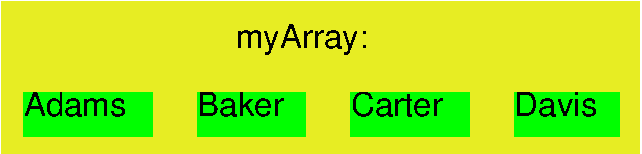
\includegraphics[scale=0.5]{images/array1}
  \end{center}
  \caption{A Sorted Array of Strings}\label{fig:sortedArrayi}.
\end{figure}
\begin{figure}
  \begin{center}
    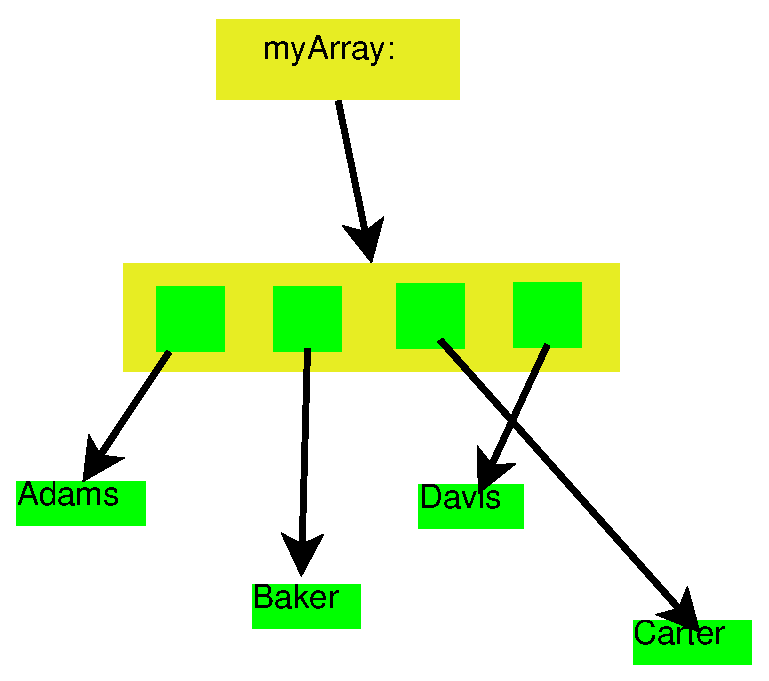
\includegraphics[scale=0.5]{images/array2}
  \end{center}
  \caption{A More Honest Sorted Array of Strings}\label{fig:sortedArrayii}.
\end{figure}

But any good Java programmer knows that \autoref{fig:sortedArrayii} is
a much more accurate portrayal of an array of strings.

Nonetheless, if I wanted to explain a sorting algorithm I would prefer
the simpler picture in \autoref{fig:sortedArrayi}. The extra pointers
are a distraction. Trying to visualize the movement of elements in the
array as shifting pointers rather than as direct rearrangements of the
data is simply not as clear.

\algae\ provides several mechanisms by which an animation designer may
opt to ``fib'' to viewers in support of better instructional
clarity. One of the most pervasive of these is in allowing the
animation designer to choose whether to present variables and data
members of objects ``inline'' or as connections/references.

Another way in which a designer may ``fib'' to viewers is to
selectively rewrite the source code displayed during the animation, as
we will see shortly.

\subsection{Inserting Breakpoints}

The animation at the end of \autoref{displayingGlobal} shows only the
final outcome of executing each function. We can see, for example,
that each of the sorting algorithms does indeed sort the array, but we
are not able to follow the intermediate steps of each sorting
algorithm.

The solution is to introduce breakpoints into the sorting algorithms.
More specifically, there are two steps:
\begin{enumerate}
\item Create a (simulated) activation record for each function
\item Use that activation record to create breakpoints.
\end{enumerate}
An activation record is created by the call \texttt{Animation.activate(\ldots)}. A breakpoint is created by the activation record's member function \texttt{breakHere(\ldots)}. Here, for example, we can see the process of creating an activation record for the bubble sort function and setting a breakpoint at the very start of that function:
\begin{lstlisting}[language=Java,frame=tb]{}
public static//!
void bubbleSort(int list[], int length)
{
`\fxl{2}`  ActivationRecord arec = Animation.activate(Sorting2.class);//!
  arec.breakHere("starting bubble sort");//!
\end{lstlisting}
\begin{itemize}
\item The parameter to the \texttt{activate} function fulfills two purposes:
  \begin{enumerate}
  \item It helps the source code viewer to locate the appropriate file of
    source code.
  \item If it is supplied with a \texttt{this} reference (in a non-static member function), then that parameter is also displayed as part of the visible rendering of the activation stack.

    In this case, the function being animated is static, so we supply the class object instead of a \texttt{this} reference.
  \end{enumerate}

  \item The parameter to the \texttt{breakHere()} function is a
    descriptive string that is displayed on the status line when the
    breakpoint is encountered. Use these strings to establish a
    running commentary on the progress of the algorithm:
\begin{lstlisting}[language=Java,frame=tb]{}
public static//!
void bubbleSort(int list[], int length)
{
    ActivationRecord arec = Animation.activate(Sorting2.class);//!
`\fxl{1}`    arec.breakHere("starting bubble sort").show();//!
    int temp;
    int iteration;
    int index;

    for (iteration = 1; iteration < length; iteration++)
    {
`\fxl{1}`        arec.breakHere("start a pass over the array");//!
        for (index = 0; index < length - iteration; index++)
        {//!
`\fxl{1}`            arec.breakHere("compare list[index] to list[index+1]");//!
            if (list[index] > list[index + 1]) 
            {
`\fxl{1}`                arec.breakHere("list[index] and list[index+1] are out of order - swap them");//!
                temp = list[index];
                list[index] = list[index + 1];
                list[index + 1] = temp;
            }
        }//!
`\fxl{1}`        arec.breakHere("completed this pass over the array");//!

    }
`\fxl{1}`    arec.breakHere("completed bubble sort");//!
}
\end{lstlisting}
\end{itemize}

Many of the statements in the above listing end with the comment
marker \texttt{//!}. This marker is a signal for selective rewriting
by the source code viewer.
\begin{itemize}
\item For any source code line that contains a \texttt{//!}, the
  source code viewer will not display the part of that line from the
  start of the line up to and including the \texttt{//!}.
\item If the remaining part of the line after a \texttt{//!} has no
  non-whitespace characters, then the entire line is omitted from the
  source code viewer.
\end{itemize}
The statements that create the activation records and the breakpoints
are terminated with a \texttt{//!} marker so that they are never shown
to the students running the animation. This is an example of pnambic
(Pay No Attention to the Man BehInd the Curtain) behavior
\cite{pnambic}, or, as I have described it earlier, the fine art of
fibbing to the students for instructional purposes.

This version of the system (including breakpoints in all three sorting algorithms) can be executed (within the reference manual project
directory) as \texttt{SortingDriver2}. You can see that the individual changes to the array are visible at each step.


\subsection{Displaying Local Data}

The most recent version of the animation still does not provide enough
information to allow students to understand what is happening. The
primary problem now is that the array is the {\em only} data being
shown. But understanding the behavior of these algorithms depends on
knowledge of the values of the various indices, loop counters, and
temporary variables used within the algorithm.

To add local data to the display, we register desired variables or expressions with the breakpoint. There are two kinds of local data to be displayed: parameters and variables.

For example, this code
\begin{lstlisting}[language=Java,frame=tb]{}
public static//!
    void bubbleSort(int list[], int length)
    {
     ActivationRecord arec = Animation.activate(Sorting3.class);//!
`\fxl{1}`     arec.refParam("list", list).param("length", length).breakHere("starting bubble sort");//!
\end{lstlisting}
adds two parameters to the display of the breakpoint.
\begin{itemize}

\item In this case, we have opted to display the \texttt{list} parameter as a pointer (because the array itself is already being displayed as a global variable. The \texttt{length} parameter, however, is displayed inline (\autoref{parameterDisplay}).

\item The two
parameters are labeled ``list'' and ``length'' (matching the formal
parameter names of the function) and the actual values of these
parameters are also passed in each call.



\item It's convenient, but not necessary to combine all the breakpoint manipulation into one line.  It could be broken up:
\begin{lstlisting}[language=Java,frame=tb]{}
public static//!
    void bubbleSort(int list[], int length)
    {
     ActivationRecord arec = Animation.activate(Sorting3.class);//!
`\fxl{3}`     arec.refParam("list", list);//!
     arec.param("length", length)//!
     arec.breakHere("starting bubble sort");//!
\end{lstlisting}

\end{itemize}


\begin{figure}
  \begin{center}
    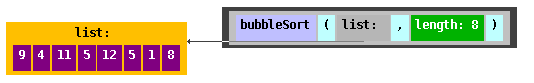
\includegraphics[scale=0.5]{images/parameterDisplay}
  \end{center}
  \caption{Displaying Parameters of a Call}\label{parameterDisplay}
  
\end{figure}

As we advance further into the algorithm, we add the second type of
local display -- variables:
\begin{lstlisting}[language=Java,frame=tb]{}
public static//!
    void bubbleSort(int list[], int length)
    {
       ActivationRecord arec = Animation.activate(Sorting3.class);//!
       arec.refParam("list", list).param("length", length).breakHere("starting bubble sort");//!
       int temp;
       int iteration;
       int index;

       for (iteration = 1; iteration < length; iteration++)
       {
`\fxl{1}`           arec.var("iteration", iteration);//!
           arec.breakHere("start a pass over the array");//!
           for (index = 0; index < length - iteration; index++)
           {//!
`\fxl{1}`               arec.var("index", index);//!
               arec.breakHere("compare list[index] to list[index+1]");//!
               if (list[index] > list[index + 1]) 
               {
                  arec.breakHere("list[index] and list[index+1] are out of order - swap them");//!
                  temp = list[index];
                  list[index] = list[index + 1];
                  list[index + 1] = temp;
                }
           }//!
           arec.breakHere("completed this pass over the array");//!

       }
       arec.breakHere("completed bubble sort");//!
    }
\end{lstlisting}
\begin{itemize}
\item The \texttt{var()} calls are similar to those for registering parameters, but variables will be displayed outside of the call stack.
\item Again, the two parameters for each variable registration consist of a name for the variable to display and a value to be displayed (\autoref{localVars}).
\item Although not used here, we also have the option of displaying a local variable as a reference arrow to a separately allocated object. The call for doing so is called \texttt{refVar()}.
\end{itemize}
\begin{figure}
  \begin{center}
    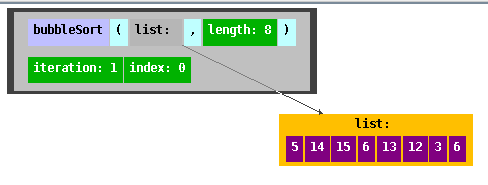
\includegraphics[scale=0.5]{images/localVars}
  \end{center}
  \caption{Displaying Local Variables}\label{localVars}
  
\end{figure}


What, precisely, does the \algae\ syetem ``remember'' when a parameter or variable is registered?  It remembers the reference value stored in the registered value. So, when we say, for example,
\begin{lstlisting}[language=Java,frame=tb]{}
public static//!
    void bubbleSort(int list[], int length)
    {
       ActivationRecord arec = Animation.activate(Sorting3.class);//!
       arec.refParam("list", list).param("length", length).breakHere("starting bubble sort");//!
\end{lstlisting}
what is registered for the parameter ``list'' is the reference
(address) stored in the variable \texttt{list}. For the parameter
``length'', things are a touch more complicated. \texttt{length} is a primitive (int) variable. It does not contain a refernece. However, when \texttt{param(\ldots)} or the other registration functions are called, Java will automatically convert the \texttt{int} value to an \texttt{Integer} object, and it will be the address of that temporary variable that is remembered.

All this is fine as long as the value of the primitive does not change (or, in general, as long as the reference stored in a parameter or variable does not change).  So \texttt{list} is fine -- its value changes but its address does not. \texttt{length} is also fine -- the sorting algorithm does not change the value of this primitive.

Looking down a little further, though we see the local variables \texttt{iteration} and \texttt{index}, which \textit{do} change value repeatedly.
\begin{lstlisting}[language=Java,frame=tb]{}
 public static//!
    void bubbleSort(int list[], int length)
    {
        ActivationRecord arec = Animation.activate(Sorting3.class);//!
        arec.refParam("list", list).param("length", length).breakHere("starting bubble sort");//!
        int temp;
        int iteration;
        int index;

`\fxl{1}`        for (iteration = 1; iteration < length; iteration++)
        {
`\fxl{1}`            arec.var("iteration", iteration);//!
            arec.breakHere("start a pass over the array");//!
`\fxl{1}`            for (index = 0; index < length - iteration; index++)
            {//!
`\fxl{1}`                arec.var("index", index);//!
                arec.breakHere("compare list[index] to list[index+1]");//!
                if (list[index] > list[index + 1]) 
                {
                    arec.breakHere("list[index] and list[index+1] are out of order - swap them");//!
                    temp = list[index];
                    list[index] = list[index + 1];
                    list[index + 1] = temp;
                }
            }//!
            arec.breakHere("completed this pass over the array");//!

        }
        arec.breakHere("completed bubble sort");//!
    }
\end{lstlisting}
When a primitive changes value or an object variable changes its
reference value, then we must re-register it using the same param/var
function and the same label. The new value then replaces the old
one. In this case, \texttt{iteration} and \texttt{index} are
re-registered at the start of each iteration of their respective
loops, which corresponds to the only times at which their values
change.

One last detail remains to be considered. Once registered for display, a parameter or variable will normally be displayed until execution returns from the function. That's not always appropriate. For example, the last registered values of \texttt{iteration} and \texttt{index} would be displayed at the final, ``completed bubble sort'' although, technically, neither variable exists outside of their respective loops.  You can designate a more limited lifetime for displayed variables by creating and destroying a ``scope'' over the relevant portion of the program. 
\begin{lstlisting}[language=Java,frame=tb]{}
 public static//!
    void bubbleSort(int list[], int length)
    {
        ActivationRecord arec = Animation.activate(Sorting3.class);//!
        arec.refParam("list", list).param("length", length).breakHere("starting bubble sort");//!
        int temp;
        int iteration;
        int index;

        for (iteration = 1; iteration < length; iteration++)
        {
`\fxl{1}`            arec.pushScope();//!
            arec.var("iteration", iteration);//!
            arec.breakHere("start a pass over the array");//!
            for (index = 0; index < length - iteration; index++)
            {//!
`\fxl{1}`                arec.pushScope();//!
                arec.var("index", index);//!
                arec.breakHere("compare list[index] to list[index+1]");//!
                if (list[index] > list[index + 1]) 
                {
                    arec.breakHere("list[index] and list[index+1] are out of order - swap them");//!
                    temp = list[index];
                    list[index] = list[index + 1];
                    list[index + 1] = temp;
                }
`\fxl{1}`                arec.popScope();//!
            }//!
            arec.breakHere("completed this pass over the array");//!

`\fxl{1}`            arec.popScope();//!
        }
        arec.breakHere("completed bubble sort");//!
    }
\end{lstlisting}


Any new variables introduced after a \texttt{pushScope} call are forgotten upon execution of the matching \texttt{popScope} call.



This version of the system (including parameters and local variables
in all three sorting algorithms) can be executed (within the reference
manual project directory) as \texttt{SortingDriver3}. This is now an
animation that could be useful to students trying to learn these
algorithms.




\subsection{Decoration}

Although potentially useful, the prior version of the sorting demo is
still not quite as clear as we might wish. Understanding what is going
on with array manipulation requires mentally correlating the values of
various indices against the data in corresponding positions in the
array. Even with relatively small arrays, it can be easy to slip up.

Sometimes it is useful to add explicit {\em decoration} to a
breakpoint that can focus the viewer's attention on specific data
elements.

Two useful ways to add decorations are by adding connections to the
diagram or by exploiting color changes.



\subsubsection{Decorative Connections}

The package \texttt{edu.odu.cs.zeil.AlgAE.Utilities} contains, among
other things, a number of {\em wrapper} (a.k.a. {\em adapter}) classes
\cite{Gamma/patterns} for data that ``indexes'' into other
collections. These include wrappers for Java iterators and, the one
that we will use, an \texttt{Index} wrapper for integers that are used
to index into one or possibly two different arrays or {\tt Iterable}
structures.

An index is created via a constructor that takes two parameters. The
first is the integer value of the index, and the second is the array
or {\tt java.util.Iterable} container that it indexes into. An {\tt
Index} is rendered like an integer value but with a colored arrow
pointing to the component of the array/container indicated by that
position value.

Here I have decorated both the {\tt index} and {\tt smallestIndex} variables in the bubble sort:
\begin{lstlisting}[language=Java,frame=tb]{}
    public static//!
    void bubbleSort(int list[], int length)
    {
        ActivationRecord arec = Animation.activate(Sorting3.class);//!
        arec.refParam("list", list).param("length", length).breakHere("starting bubble sort");//!
        int temp;
        int iteration;
        int index;

        for (iteration = 1; iteration < length; iteration++)
        {
            arec.pushScope();//!
`\fxl{1}`            arec.var("iteration", new Index(iteration, list));//!
            arec.breakHere("start a pass over the array");//!
            for (index = 0; index < length - iteration; index++)
            {//!
                arec.pushScope();//!
`\fxl{1}`                arec.var("index", new Index(index, list));//!
                arec.breakHere("compare list[index] to list[index+1]");//!
                if (list[index] > list[index + 1]) 
                {
                    arec.breakHere("list[index] and list[index+1] are out of order - swap them");//!
                    temp = list[index];
                    list[index] = list[index + 1];
                    list[index + 1] = temp;
                }
                arec.popScope();//!
            }//!
            arec.breakHere("completed this pass over the array");//!

            arec.popScope();//!
        }
        arec.breakHere("completed bubble sort");//!
    }
\end{lstlisting}
so that each will be shown pointing to the specific element of the {\tt list} array that is being referenced.


This version of the sorting demo can be executed (within the reference
manual project directory) as \texttt{SortingDriver4}. This is, by and large,
the version that I actually distributed to my class.


\subsubsection{Decorative Color}

Color changes can also be an effective way to draw a viewer's
attention to a specific group of objects.  The
\texttt{ActivationRecord} class supports operations {\tt
  highlight(object)} and {\tt highlight(object, color)} to create
temporary color changes. Their effects will end upon returning from
the current function and will be suspended during calls from that
function. (Permanent color changes are discussed later in
\autoref{rendering}.)

For example, in the {\tt insertionSort}, we might consider
highlighting the element being compared against the temp value and
also using a fixed color to distinguish the already sorted portion of
the array from the portion that has not been checked:
\begin{lstlisting}[language=Java,frame=tb]{}
public static//!
    void insertionSort (int list[], int listLength)
    {
        ActivationRecord arec = Animation.activate(Sorting3.class);//!
        arec.refParam("list", null).param("listLength", listLength);//!
        arec.breakHere("starting insertion sort");//!
        int firstOutOfOrder, location;
        int temp;
        
        for (firstOutOfOrder = 1; firstOutOfOrder < listLength;
                                  firstOutOfOrder++)
        {//!
            arec.var("firstOutOfOrder", new Index(firstOutOfOrder, list));//!
            arec.breakHere("move list[firstOutOfOrder] into place");//!
            if (list[firstOutOfOrder] < list[firstOutOfOrder-1])
            {
                temp = list[firstOutOfOrder];
                location = firstOutOfOrder;
                arec.var("temp",temp).var("location", new Index(location, list));//!
                arec.breakHere("temp holds the value we want to insert");//!
                
                do
                {
`\fxl{1}`                    arec.highlight(list[location-1]);//!
                    arec.breakHere("shift an element up to make room");//!
                    list[location] = list[location - 1];
`\fxl{1}`                    arec.breakHere("then move to the next lower element");//!
                    arec.highlight(list[location-1]);//!
                    location--;
                    arec.var("location", new Index(location, list));//!
                    }
                while (location > 0 && list[location - 1] > temp);
                
                arec.breakHere("Now we know where to insert temp");//!
                list[location] = temp;
`\fxl{1}`                arec.highlight(list[location], Color.lightGray);//!
            }
            arec.breakHere("Move to the next unordered element");//!
        }//!
        arec.breakHere("Completed insertion sort");//!
    }
\end{lstlisting}
\begin{itemize}
\item If no color parameter is specified, the \texttt{highlight}
  function ``inverts'' the color of the object: i.e., if the RBG
  colors are expressed on a $0.0\ldots 1.0$ scale, then an object of
  color $(r,g,b)$ is changed to color $(1-r,1-g,1-b)$.
  \begin{itemize}
  \item Consequently, highlighting the same object a second 
    time actually returns it to its original color.
  \end{itemize}
\item Alternatively, an explicit color can be selected 
  in a highlight parameter.
\end{itemize}

Unfortunately, the change shown here will actually have no visible
effect.  That's because all renderable objects actually need to {\bf
  be} objects. When we pass an {\tt int} or other non-class primitive,
they are converted to a corresponding {\tt Integer} or other container
object. That converted object is what is actually being shown, and
because we don't have a reference to that object, we can't pass it to
a \texttt{highlight} call.

A possible solution is to actually change the array supplied by the
driver from an array of {\tt int} to and array of {\tt Integer}:
\begin{lstlisting}[language=Java,frame=tb]{}
public class SortingDriver5 extends Animation {

    public SortingDriver5() {
        super("Sorting Algorithms", true);
    }

    @Override
    public String about() {
        return "Demonstration of Sorting Algorithms,\n" +
                "prepared for CS 333, Advanced Data Structures\n" +
                "and Algorithms, Old Dominion University\n" +
                "Summer 2011";
    }

    
`\fxl{1}`    private Integer[] array = new Integer[8];
       `\vdots`
\end{lstlisting}

This, however, requires that the sorting functions be rewritten to
work with an array of {\tt Integer} as well. The resulting changes
are probably not something we want the viewers to see, so we must engage in
some selective rewriting of the source code:
\begin{lstlisting}[language=Java,frame=tb]{}
public class Sorting5 {//!
    `\vdots`
void bubbleSort(Integer list[], int length)//!	void bubbleSort(int list[], int length)
    `\vdots`
void selectionSort(Integer list[], int length)//!	void selectionSort(int list[], int length)
    `\vdots`
void insertionSort (Integer list[], int listLength)//!	void insertionSort (int list[], int listLength)
    `\vdots`
}//!
\end{lstlisting}

\begin{figure}
  \begin{center}
    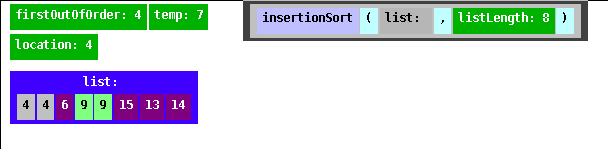
\includegraphics[scale=0.5]{images/IntegerAliasing}
  \end{center}
  \caption{Unintended Aliasing}\label{IntegerAliasing}
  
\end{figure}

This is easy enough, but it also runs into problems on some(?) Java
engines.  You will almost certainly discover that whenever one element
in the array is highlighted, any elements containing the same value
will also be highlighted (See \autoref{IntegerAliasing}).

The problem is that, despite being rendered as distinct components of
the array, the array is actually holding references to the actual
values on the heap, and, in this case, some pairs of those are
actually shared references to the same object. Consequently,
highlighting the one object shared by two different array elements
causes all of those array elements to appear highlighted.

Now that is a common problem that can arise when designing an
animation, but, if you examine the Sorting Demo code closely, you may
be at a loss to find the reason for this sharing. In fact, there's
some rather strange behavior associated with the Java \texttt{Integer}
class. The program in \autoref{list:integerAliasing} reveals that some
sort of caching is used when \texttt{int} values are converted
implicitly to \texttt{Integer}, with the result that \texttt{Integer}
containers holding equal {\tt int} values will often occupy the same
address.

\lstinputlisting[language=Java,frame=TB,caption={Integers Are Shared Unexpectedly\label{list:integerAliasing}}]{src/IntegerAliasing.java}

When run with Oracle Java 1.6, this program produces the output
\begin{verbatim}
The two arrays share 100 elements.
\end{verbatim}


To counter this problem, the \texttt{edu.odu.cs.zeil.AlgAE.Utilities}
contains a \texttt{DiscreteInteger} container in which no such sharing
will occur. \texttt{DiscreteInteger}s are also mutable, making them a
better fit for many algorithms. On the other hand, they do not get the
benefit of implicit conversion to and from \texttt{int}, so the use of
\texttt{DiscreteInteger} would require more rewriting of the sorting
algorithms and still more selective rewriting of the source code.

In practice, I generally find that decoration of algorithms takes far
more time and effort than does getting a basic animation with
breakpoints and rendering of data.  You therefore want to be careful
in pursuing decorations, restricting their use to situations where they
truly enhance the instructional role of the animation.



\section{Rendering Your Own Structures}\label{rendering}

The sorting demo that formed the basis of the previous section had a
major simplification that won't always be available. The only data
being drawn were primitives such as \texttt{int} values and
arrays. \algae\ ``knows'' how to render these types (and a good
handful of other types including \texttt{String}s and anything that
implements \texttt{Iterable}.

In this section, we will consider the problem of portraying a new class
type for which no acceptable set of rendering rules has yet been
provided.

The starting point for this discussion will be code for inserting an element into a singly linked list:
\begin{lstlisting}[language=Java,frame=tb]{}
package edu.odu.cs.AlgAE.Demos;//!

public class SinglyLinkedLists {


  class nodeType
  {
      int info;
      nodeType link;

      public nodeType()
      {
          link = null;
      }
  }


  private nodeType head = null;


  public void addToFront (int k)
  {
     nodeType newNode = new nodeType();
     newNode.link = head;
     newNode.info = k;
     head = newNode;
  }

  public void insert (nodeType p, int value)
  {
     nodeType newNode = new nodeType();
     newNode.info = value;
     newNode.link = p.link;
     p.link = newNode;
  }
     
}
\end{lstlisting}

In this example, we will be interested only in demonstrating the process of inserting a node into a linked list, so the driver will provide only a single menu item:

\lstinputlisting[language=Java,frame=TB,caption={Driver For Singly-Linked List Insertion\label{list:sllDriver}}]{src/edu/odu/cs/AlgAE/Demos/SLLInsertionDriver0.java}

We can also start with a set of breakpoints in the insertion function.
\lstinputlisting[language=Java,frame=TB,caption={Singly-Linked List Insertion Breakpoints\label{list:sllBP}}]{src/edu/odu/cs/AlgAE/Demos/SinglyLinkedLists0.java}

\begin{figure}
  \begin{center}
    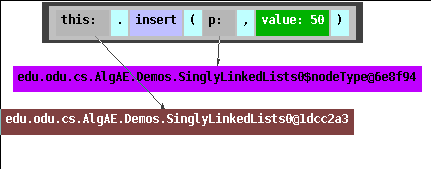
\includegraphics[scale=0.5]{images/noRendering}
  \end{center}
  \caption{Singly-Linked Lists: Default Rendering}\label{fig:noRendering}
  
\end{figure}

Running this animation (\texttt{SLLInsertionDriver0}) yields disappointing results (\autoref{fig:noRendering}). That's because we have supplied no rendering options for the two data types (\texttt{SinglyLinkedLists} and \texttt{SinglyLinkedLists.nodeType}) being displayed. Consequently, the default rendering rules are being applied.

\subsection{Rendering}

\algae\ {\em renders} objects according to five criteria:
\begin{enumerate}
\item What color should be used for the enclosing box?
\item What are the components of the object?
\item How many components should be laid out per row?
\item To what other objects does this one connect?
\item What string represents the value of this object?
\end{enumerate}

For each object, \algae\ consults a chain of {\em renderers}, each of
which either provides an answer to these questions or responds with a
``don't know'' value, in which case the question is referred further
on down the chain.

Each renderer must implement this interface:
\begin{lstlisting}[language=Java,frame=tb]{}
package edu.odu.cs.zeil.AlgAE.Snapshot.Rendering;

import java.awt.Color;

/**
 * Determines how a given object or class of objects should be drawn.
 * 
 * @author zeil
 *
 */
public interface Renderer<T> {
	
	/**
	 * What string will be used as the value of this object?
	 * 	
	 * @param obj: object to be drawn
	 * @return a string or null to yield to other renderers
	 */
	public String getValue(T obj);
	
	/**
	 * What color will be used to draw this object?
	 * 	
	 * @param obj: object to be drawn
	 * @return a color or null to yield to other renderers
	 */
	public Color getColor(T obj);
	
	/**
	 * Get a list of other objects to be drawn inside the
	 * box portraying this one.
	 * 	
	 * @param obj: object to be drawn
	 * 
	 * @return an array of contained objects or null to yield to other renderers
	 */
	public List<Component> getComponents(T obj);
	
	/**
	 * Get a list of other objects to which we will draw
	 * pointers from this one.
	 * 	
	 * @param obj: object to be drawn
	 * 
	 * @return an array of referenced objects or null to yield to other renderers
	 */
	public List<Connection> getConnections(T obj);
	

	/**
	 * Indicates how components will be laid out within the box
	 * representing this object.  A return value of 1 will force all
	 * components to be laid out in a single vertical column. Larger
	 * return values will permit a more horizontal layout.
	 * 
	 * A zero value requests that components be laid out in a (more or less) minimal area.
	 * 
	 * @param obj
	 * @return max #components per row or a negative value to yield to other renderers 
	 */
			
	public int getMaxComponentsPerRow(T obj);
	
}
\end{lstlisting}
Each of the functions in this interface directly pertains to one of the 5 rendering criteria listed above.

There are several ways to associate a renderer with a particular object:
\begin{itemize}
\item An {\em object renderer} is associated with a specific object reference. Object renderers have a limited lifetime. They are created via an \texttt{ActivationRecord} and last only as long as that function activation is in effect. 

Color highlighting is actually a shorthand for creating a renderer that specifies a color but answers ``don't know'' to every other rendering question.

Object renderers have the highest priority of any kind of renderer.

\item If a rendering question cannot be resolved by an object renderer, then a search is made for a {\em type renderer} that is bound to the data type of the object or to to one of its base classes.

Type renderers can be bound in one of two ways. The most general way is for an animation driver to call \texttt{algae().render({\em classObject}, {\em renderer});}. A convenient shorthand, however, is for a type to implement the {\em CanBeRendered} interface:
\begin{lstlisting}[language=Java,frame=tb]{}
package edu.odu.cs.zeil.AlgAE.Snapshot.Rendering;

public interface CanBeRendered<T> {
   public Renderer<T> getRenderer();
}
\end{lstlisting}

in which case each object of that type supplies a reference to its 
own type renderer.  Some classes may implement both \texttt{CanBeRendered} and \texttt{Renderer}, in which case \texttt{getRenderer()} will simply return \texttt{this}.

\item  If no object renderer nor type renderer responds to a 
  particular rendering question, then the final fallback is the 
  {\em default renderer}, which behaves as follows:
  \begin{enumerate}
  \item Color: A color is selected based upon a hash of the type name. In
    essence, the color is chosen randomly, but all objects of the same
    type will have the same color.
  \item Components: If the object is an array or implements
    \texttt{Iterable}, its elements are shown as internal
    components. Otherwise, the object has no components.
  \item Layout: Most objects are arranged vertically (1 component per
    row).  However, arrays alternate horizontal and vertical depending
    on dimensionality. A one-dimensional array is laid out
    horizontally (100 elements per row), a two dimensional array is
    laid out as a vertical list of one-dimensional rows, and so on.
  \item Connections: none
  \item Value: Determined by calling \texttt{toString()}

    Not that this provides a useful default for primitives, Strings,
    and many other classes. \autoref{fig:noRendering}, however, shows
    that a class that provides no renderer of its own {\em and} that
    fails to implement \texttt{toString()} will yield rather ugly
    results.
  \end{enumerate}

\end{itemize}

\subsection{Rendering Linked List Nodes}

Let's start, then, by creating a renderer for the inner \texttt{nodeType} class from \autoref{list:sllBP}.

To make this easy, we will use the \texttt{CanBeRendered} approach
(although this increases the number of lines of code we will need to
hide with \texttt{//!}).

We will start by having the node type declare that it will provide its own renderer:
\begin{lstlisting}[language=Java,frame=tb]{}
class nodeType 
`\fxl{1}`implements CanBeRendered<nodeType>, Renderer<nodeType>//!
{
    int info;
    nodeType link;
    
    public nodeType()
    {
`\fxl{1}`    	info = -999;//!
    	link = null;
    }

    public Renderer<nodeType> getRenderer() {//!
        return this;//!
    }//!
      `\vdots`
\end{lstlisting}

Now, how shall we actually render this?  
\begin{enumerate}
\item We'll choose any color that we like:
\begin{lstlisting}[language=Java,frame=tb]{}
      `\vdots`
    public Color getColor(nodeType obj) {//!
        return Color.green.darker();//!
    }//!
      `\vdots`
\end{lstlisting}

\item Each node will have a single internal component, its \texttt{info} field.
\begin{lstlisting}[language=Java,frame=tb]{}
      `\vdots`
    public List<Component> getComponents(nodeType obj) {//!
        LinkedList<Component> data = new LinkedList<Component>();//!
        data.add (new Component(info, "info"));//!
        return data;//!
    }//!
      `\vdots`
\end{lstlisting}
Actually, we could just as easily treat this as the ``value'' string
of the object, but treating it as a separate component is more
flexible in case we later want to adapt this code to lists of other
kinds of data.

Components can be given optional labels (e.g., ``info'' in this
case). in which case those labels will appear within the
rendering. One might commonly use such labels for components
representing a single data member while eschewing any such labels for
components of a more array-like structure.


\item The \texttt{link} field will supply the only connection 
leaving this object.
\begin{lstlisting}[language=Java,frame=tb]{}
      `\vdots`
    public List<Connection> getConnections(nodeType obj) {//!
        LinkedList<Connection> links = new LinkedList<Connection>();//!
        Connection c =  new Connection(link, 85.0, 95.0);//!
        c.setLabel("link");//!
        links.add(c);//!
        return links;//!
    }//!
      `\vdots`
\end{lstlisting}
When creating connections, we give a range of angles from which the
connection may emerge. In this case, I use the range from 85 to 95
degrees. Zero degrees represents straight up vertically, and 90
degrees points directly to the right.

These angles have a tremendous effect upon the rendering of connected
entities. Consider, for example, that a typical doubly-linked list
node and a typically binary tree node are topologically identical -
each has a data field and a pair of emerging pointers. But if those
pointers emerge at opposite ends of the node (90 and 270 degrees),
then the nodes will tend to arrange themselves into a straight
line. If those pointers emerge from the bottom corners (135 and 225
degrees), then even a fairly degenerate tree will try to arrange itself
into the traditional ``inverted-Vs'' drawing.

\item Since we only have one internal component, the number of components per row is largely irrelevant:
\begin{lstlisting}[language=Java,frame=tb]{}
      `\vdots`
    public int getMaxComponentsPerRow(nodeType obj) {//!
        return 100;//!
    }//!
      `\vdots`
\end{lstlisting}

\item And we won't need an explicit value string, because we have opted to show the \texttt{info} as a nested component.
\begin{lstlisting}[language=Java,frame=tb]{}
      `\vdots`
    public String getValue(nodeType obj) {//!
        return "";//!
    }//!
\end{lstlisting}
\end{enumerate}

With these rendering functions, and a similar but even simpler set for the \texttt{SinglyLinkedLists} class itself, we arrive at an animation (SLLInsertionDriver) that produces images such as in \autoref{fig:sllrender}.

\begin{figure}
  \begin{center}
    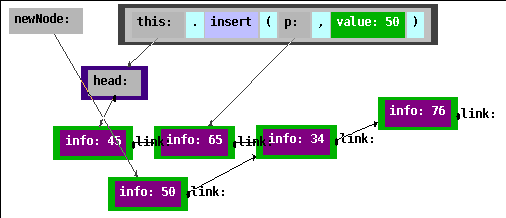
\includegraphics[scale=0.5]{images/sllrender}
  \end{center}
  \caption{Singly-Linked Lists: Rendering}\label{fig:sllrender}
  
\end{figure}



\section{Continuous Animations}\label{looping}

The linked list insertion demo is rather limited, as it runs only a
single algorithm. The reason for this is that it was actually
originally intended as an applet that would be embedded (inline) into a course
web page devoted to that specific algorithm.

For that purpose, it might be useful if the algorithm ran 
itself immediately and continuously as soon as the web page was visited.

This can be accomplished by making calls to the animated function from
the starting action, the \texttt{MenuFunction} called before any
choices are offered to the viewer. In the driver, we add a new registration:
\begin{lstlisting}[language=Java,frame=tb]{}
      `\vdots`
    @Override
    public void buildMenu() {

`\fxl{15}`        registerStartingAction(new MenuFunction() {
            @Override
            public void selected() {
                getAnimator().setSpeed(30);
                for (int k = 0; k < 1000; ++k) {
                    generateLL();                    
                    sll.insert(sll.head.link, 50);
                    try {
                        Thread.sleep(2500);
                    } catch (InterruptedException e) {
                        break;
                    }
                }
            }    
        });

        
        register ("Insert a node", new MenuFunction() {

            @Override
            public void selected() {
                generateLL();                    
                sll.insert(sll.head.link, 50);
            }
            
        });
      `\vdots`
\end{lstlisting}
\begin{itemize}
\item Normal menu selections start with the viewer in pausing mode -
  it will stop at each breakpoint. The starting action, however, runs
  by default in continuous mode. The optional \texttt{setSpeed} call
  is used to slow down the default speed with which it moves from
  breakpoint to breakpoint.

\item  Similarly, the \texttt{sleep} call at the end helps inject a 
  slight pause between each restart of the algorithm.

\item Rather than looping forever, I prefer to use a loop like the for loop shown here to repeat the demonstration a large but finite number of times. The regular Algorithm menu function can be kept available if someone were to stay on the page long enough for this loop to complete.
\end{itemize}



\section{User Interaction}\label{interaction}

Because \algae\ is actually executing the code being animated, rather
than simply displaying a pre-determined sequence of pictures, an
\algae\ animation can accept user inputs and demonstrate how the
algorithm would react to those.

For example, we might alter the driver for the (non-continuous) linked list insertion function as follows:
\begin{lstlisting}[language=Java,frame=tb]{}
      `\vdots`
    @Override
    public void buildMenu() {
        register ("Insert a node", new MenuFunction() {

            @Override
            public void selected() {
                generateLL();
`\fxl{3}`                String val = promptForInput("What number to insert?", "[0-9]+");
		int value = Integer.parseInt(val);
                sll.insert(sll.head.link, value);
            }
            
        });
      `\vdots`
\end{lstlisting}
\begin{itemize}
\item The \texttt{promptForInput} function takes two parameters. The
  first is a prompt string that is displayed in a pop-up activation
  box. The second is a regular expression describing a valid input
  string. If the user responds with a string that does not match this
  pattern, he or she will be prompted again for a new input.
\item Another mechanism for interaction is provided by the I/O streams
  \texttt{Animation.in} and \texttt{Animation.out}, which can be
  thought of as analogues of the more conventional \texttt{System.in} and
  \texttt{System.out}.
  These streams, however, read and write from the I/O pane located in 
  the lower right of the animation (\autoref{session}).
\end{itemize}






\chapter{Animating a \cpp\ Algorithm}

Version 3.0 of \algae\ no longer supports direct animation of
\cpp\ code. I hope to restore this ability in the near future.

However, by using the selective rewriting facility of the
source code viewer, one can easily portray a set of animated Java
algorithms as \cpp, as pseudo-code, or as almost any other language.
\cpp\ is a particularly easy case because so much code in that
language is also valid Java code.

For example, for one of my classes I wished to animate the following
sorting algorithms taken from the course textbook \cite{Malik/text}:
\begin{lstlisting}[language=C++]{}
void bubbleSort(int list[], int length)
{
    int temp;
    int iteration;
    int index;

    for (iteration = 1; iteration < length; iteration++)
    {
        for (index = 0; index < length - iteration; index++)
            if (list[index] > list[index + 1]) 
            {
                temp = list[index];
                list[index] = list[index + 1];
                list[index + 1] = temp;
            }
    }
}

void selectionSort(int list[], int length)
{
    int index;
    int smallestIndex;
    int location;
    int temp;

    for (index = 0; index < length - 1; index++)
    {
            //Step a
        smallestIndex = index; 

        for (location = index + 1; location < length; location++)
            if (list[location] < list[smallestIndex])
                smallestIndex = location; 

            //Step b
        temp = list[smallestIndex];
        list[smallestIndex] = list[index];
        list[index] = temp;
    }
}


void insertionSort (int list[], int listLength)
{
    int firstOutOfOrder, location;
    int temp;
        
    for (firstOutOfOrder = 1; firstOutOfOrder < listLength;
                              firstOutOfOrder++)
        if (list[firstOutOfOrder] < list[firstOutOfOrder-1])
        {
            temp = list[firstOutOfOrder];
            location = firstOutOfOrder;
                
            do
            {
                list[location] = list[location - 1];
                location--;
            }
            while (location > 0 && list[location - 1] > temp);
                
            list[location] = temp;
        }
}
\end{lstlisting}

To do this, I simply created a basic Java package structure:
\begin{lstlisting}[language=Java]{}
package edu.odu.cs.cs333.animations;//!

import edu.odu.cs.zeil.AlgAE.ActivationRecord;//!
import edu.odu.cs.zeil.AlgAE.Animation;//!

public class Sorting {//!


//
//  Based on Malik, "C++ Programming [From Problem Analysis to Program Design]"
//      chapter 10
//

   `\vdots`
}//!
\end{lstlisting}
marking the new Java statements with a trailing \texttt{//!} so that 
they would not be displayed by the source code viewer.

I then pasted the \cpp\ code into the middle of the package and added ``\texttt{public static}'' to each function.
\begin{lstlisting}[language=Java]{}
package edu.odu.cs.cs333.animations;//!

import edu.odu.cs.zeil.AlgAE.ActivationRecord;//!
import edu.odu.cs.zeil.AlgAE.Animation;//!

public class Sorting {//!


//
//  Based on Malik, "C++ Programming [From Problem Analysis to Program Design]"
//      chapter 10
//

public static//!
void bubbleSort(int list[], int length)
{
    int temp;
    int iteration;
    int index;

    for (iteration = 1; iteration < length; iteration++)
    {
        for (index = 0; index < length - iteration; index++)
            if (list[index] > list[index + 1]) 
            {
                temp = list[index];
                list[index] = list[index + 1];
                list[index + 1] = temp;
            }
    }
}

public static//!
void selectionSort(int list[], int length)
{
    int index;
    int smallestIndex;
    int location;
    int temp;

    for (index = 0; index < length - 1; index++)
    {
            //Step a
        smallestIndex = index; 

        for (location = index + 1; location < length; location++)
            if (list[location] < list[smallestIndex])
                smallestIndex = location; 

            //Step b
        temp = list[smallestIndex];
        list[smallestIndex] = list[index];
        list[index] = temp;
    }
}


public static//!
void insertionSort (int list[], int listLength)
{
    int firstOutOfOrder, location;
    int temp;
        
    for (firstOutOfOrder = 1; firstOutOfOrder < listLength;
                              firstOutOfOrder++)
        if (list[firstOutOfOrder] < list[firstOutOfOrder-1])
        {
            temp = list[firstOutOfOrder];
            location = firstOutOfOrder;
                
            do
            {
                list[location] = list[location - 1];
                location--;
            }
            while (location > 0 && list[location - 1] > temp);
                
            list[location] = temp;
        }
}

}//!
\end{lstlisting}

The resulting Java code is, in fact, the starting point for the example 
given earlier in \autoref{sortingExample}.

In many cases, the process is a little more involved than that, but
the principle remains the same.  For example, a block of C++ code to walk 
a linked list
\begin{lstlisting}[language=C++]{}
void traverse (Node* head)
{
  Node* current = head;
  while (current != 0)
    {
      cout << current->data << endl;
      current = current->next;
    }
}
\end{lstlisting}
will need to be rewritten almost entirely. Even this is not as bad as
it seems, however, because the equivalent Java code still exhibits a
one-to-one correlation among the statements:
\begin{lstlisting}[language=C++]{}
void traverse (Node head)//!void traverse (Node* head)
{
  Node current = head;//!  Node* current = head;
  while (current != null)//!  while (current != 0)
    {
      System.out.println(current.data);//!      cout << current->data << endl;
      current = current.next;//!      current = current->next;
    }
}
\end{lstlisting}
I generally start this process by using an editor with a keyboard
macro capability to put a \texttt{//!} at the beginning of each line,
then move down line by line, copying everything to the right of the
\texttt{//!}, pasting it at the start of the line, and making whatever
small changes are actually necessary.


\bibliographystyle{abbrv}
\bibliography{referenceManual}

%\input{refmanappendix.tex}
\end{document}
